% Formulation of the main problem in terms of naming game
The issue addressed by my thesis is not argumentation on meaning \emph{per se}, an argumentation being always a mean to attain a goal. And in my thesis, the goal that needs to be reached -- through an argumentation -- is the alignment of two classifiers. We want to have, as an output of our argumentation, two agents able to classify in a consistent way a set of examples called context $U$ that represents the union of the examples known by the system of agents. By consistent I mean that both agents classify each of the examples in $U$ with a same label $s$. In simpler terms, we want both agents using the same name for a same example during a naming game where the agents are presented each example of $U$ one after the other.
% What we need in order to play the naming game
If two classifiers $A_{1}$ and $A_2$ being aligned can be translated as $A_{1}$ and $A_{2}$ scoring a naming game, then the alignment task itself can be divided in two main goals: making the agents able to play the naming game, and making the agents able to optimize their score in the naming game.

% Necessity of example signs associations in order to play the naming game
\section{Sets of associations}
In the naming game, the classifier agents are presented one example at a time and each agent associates the example with a sign. If both agents have associated the example with the same sign, the agents have scored one success. Therefore, the first thing that the agents need in order to be able to play the game, is the ability to make example-signs associations.

\begin{restatable}[Example-sign association]{df}
The association between an example $e$ and a sign $s$ by an agent $A_{k}$ is noted $e \prescript{}{Ak}{\mapsto} s$.
\end{restatable}

After the presentation of a set of examples $U$ that we will call a \emph{context}, an agent $A_{k}$ will associate a sign $s$ from a \emph{lexicon} (a set of signs) $S$ to each example $e \in U$. This process results in a set of example-sign associations.

\begin{restatable}[Set of associations]{df}
A set of associations between the examples of $U = \{e_{1}, \ldots, e_{n}\}$ and the signs of $S = \{s_{1}, \ldots, s_{m}\}$ is noted as: $U \prescript{}{k}{\mapsto} S = \{ e_{1} \mapsto s_{i}, \ldots, e_{n} \mapsto s_{j}\}$.
\end{restatable}

% Classes formulated in term of example signs associations
\subsection{Classes}
Example-sign associations can be regrouped in \emph{classes}. Classes are sets of examples that are related to a unique sign among a specific set of example-sign associations.

\begin{restatable}[Class]{df}
A class $U(\mapsto s)$ is a subset of examples from $U$ such that $U(\mapsto s) =  \{e \in U | e \mapsto s \}$. A consequence of this is that the agents cannot associate zero or more than one sign(s) to an example from $U$.
\end{restatable}

If there are multiple signs associated to the examples of a set of associations, we can regroup them in \emph{polylexematic} classes. Polylexematic classes follow the same idea as the classes, but instead of being the examples associated to one sign in the set of associations, a polylexematic class is a a set of examples associated with a given set of signs in the set of associations.

\begin{restatable}[Polylexematic class]{df}
A polylexematic class $U(\mapsto \{s, \ldots, s'\})$ is a subset of examples from $U$ such that $U(\mapsto s) =  \{e \in U | e \mapsto s \vee \ldots \vee e \mapsto s' \}$. A consequence of this is that the agents cannot associate zero or more than one sign(s) to an example from $U$.
\end{restatable}

% Consistency of a set of associations
\subsection{Properties of sets of associations}
\subsubsection{Consistency}
An important notion linked to the sets of associations in the notion of consistency. A set of associations $U \mapsto S$ is said to be consistent if it maps each example from $U$ to exactly one sign from $S$. In term of classes, it means that for any pair of classes $U(\mapsto s_{i})$ and $U(\mapsto s_{j})$ in $U \mapsto S$ we have $U(\mapsto s_{i}) \cap U(\mapsto s_{j}) = \emptyset$ if and only if $U \mapsto S$ is consistent.

\begin{restatable}[Consistency]{pp}{consistent}
\label{pp:consistent}
A set of associations $U \mapsto S$ is consistent if and only if, for each example $e \in U$, there is no pair of associations $e \mapsto s$, $e \mapsto s'$ in $U \mapsto S$ such that $s \neq s'$.
\end{restatable}

\begin{restatable}[Classes in Consistent Sets]{pp}{classConsistent}
\label{pp:ClassConsistent}
In a set of associations $U \mapsto S$, each pair of classes $U(\mapsto s_{i})$, $U(\mapsto s_{j})$ in $U \mapsto S$ in $U \mapsto S$ are verifying $U(\mapsto s_{i}) \cap U(\mapsto s_{j}) = \emptyset$ if and only if $U \mapsto S$ is consistent.
\end{restatable}

\begin{restatable}[Polylexematic Classes in Consistent Sets]{pp}{polyConsistent}
\label{pp:PolyConsistent}
In a set of associations $U \mapsto S$, there are no polylexematic classes if and only if $U \mapsto S$ is consistent.
\end{restatable}

% Homogeneity of a set of associations
\subsubsection{Homogeneity}
% Not by themselves, but when a bunch of supervised learners are trying to learn over them
Another important notion linked to the sets of associations is the notion of homogeneity. Unlike the consistency, the homogeneity is not an intrinsic property of a set of associations, but a property given by its interaction with a set of supervised learners.

% Learning is made over a set of association and results in a set of associations
A supervised learning is made over a set of associations $U \mapsto S$ where each example from $U$ is an output and its associated sign from $S$ is a desired output. Once the learning is done, the learner can make new associations over any set of examples $U'$ with the lexicon $S$. We can therefore consider the result of this learning as a new set of associations $U' \mapsto' S$. Of course, a supervised learning can only occur over a consistent set of associations, therefore only consistent sets can be homogeneous.

% The sets of associations resulting from the learning and received for the learning are equal, no matter the division in two parts of the set
A set of associations $U \mapsto S$ is considered homogeneous for the set of supervised learners $A_{1}, \ldots A_{n}$ if each pair of its subsets that have $U \mapsto S$ for union results in a learning that makes each agent $A_{k} \in A_{1}, \ldots, A_{n}$ associate the examples of $U$ with the signs of $S$ as the set of associations $U \mapsto S$.
% We will formulate that
The exact definition of the homogeneous set of associations requires the presentation of further notions on example-sign associations. For this reason, we give its formalism in the next session, with Definition \ref{def:Homogeneity}.

% Reformulation of the main problem as classes alignment
\subsection{Classifier alignment as a naming game}
If two agents $A_{1}$ and $A_{2}$ wants to pass the naming game over a context $U$, they first need to make sure that they use the same lexicon $S$. Then, they need to ensure that $U \prescript{}{A1}{\mapsto} S $ and $ U \prescript{}{A2}{\mapsto} S$ are equal. With the help of classes, we can rewrite these two conditions as: for each $s \in S$, there should exist one and only one class $U(\prescript{}{-k}{\mapsto} s)$ such that $U(\prescript{}{k}{\mapsto} s) = U(\prescript{}{-k}{\mapsto} s)$. With this last formula, the desired outcome of the naming game has been formulated as the alignment of classes: we retrieve the classifier alignment as a reformulation of a success of the naming game.

\begin{figure}[t]
    \centering
    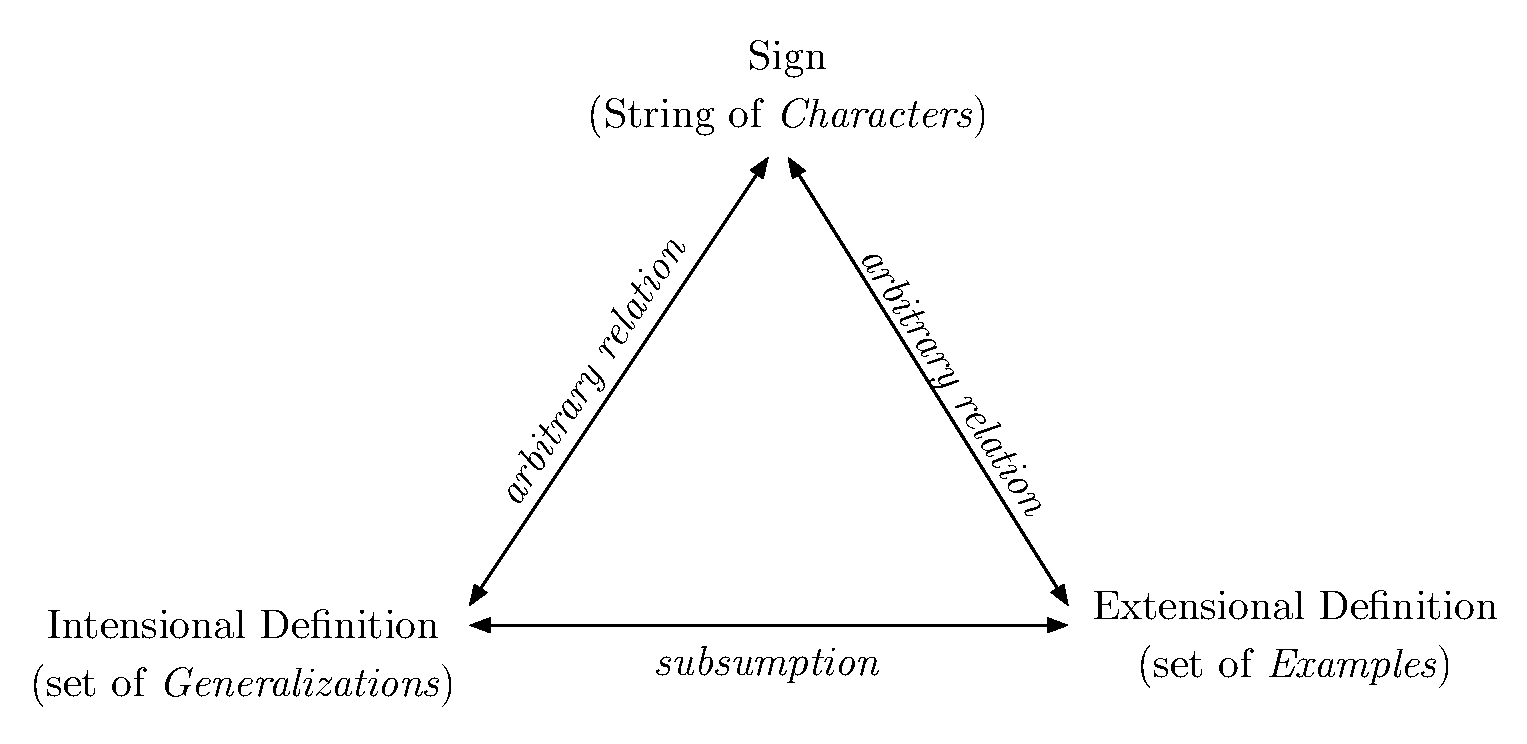
\includegraphics[width = \textwidth]{figs/4.pdf}
    \caption{The semiotic triangle and its elements}
    \label{fig:semTriangle}
\end{figure}

\section{Example-sign association}
% Presentation of the agents as inductive learner
The central element of the naming game and by extension of the classifier alignment is the example-sign association. While there are multiple ways to associate signs with examples, the agents from my thesis are classifiers that are able of supervised learning and have two main ways to make these associations.

% Present supervised learning
In supervised learning, an agent $A_{k}$ receives a \emph{consistent} set of example-sign associations $U_{k} \prescript{}{o}{\mapsto} S_{k}$ from an oracle. These associations are memorized by $A_{k}$ in a set of example-sign associations $U_{k} \prescript{}{k}{\mapsto} S_{k}$. We say that the examples $U_{k}$ are the examples that the agents have knowledge over, and are called the \emph{local} context of the agent. Comparably, the signs $S$ that an agent has knowledge over is the \emph{local} lexicon of this agent. Prior to having any supervised learning, the agent can already make example sign associations over the examples $U_{k}$ by looking up its set of example-sign associations $U_{k} \prescript{}{k}{\mapsto} S_{k}$ which constitutes an index of received example-sign associations. However, $A_{k}$ cannot make new example-sign associations.

% How the supervised learning works
The supervised learning takes place by using each example $e$ from $U_{k}$ as an input and the sign $s$ associated to $e$ in $U_{k} \prescript{}{o}{\mapsto} S_{k}$ as an expected output. Once the supervised learning is done, the agent should have learned a set of generalizations such that, provided any example $e$ and any generalization $g$, any agent could say if $e$ can be associated to $g$. Each of the generalizations that are learned are associated to a sign $s \in S_{k}$. In my thesis, the agents are inductive learners that use the feature-term formalism. The association between an example $e$ and a generalization $g$ can be tested through the relation of subsumption $g \sqsubseteq e$. The associations between examples, signs and generalizations is summarized in Figure \ref{fig:semTriangle}.

% The semiotic triangle
If we incorporate the notion of generalization to the notion of class that was already incorporating a set of examples associated to a given sign, we have a concept. A concept is is a class and the generalizations that are associated to its examples and its sign. Concepts are often represented as semiotic triangles, with their set of generalizations called the intensional definition and their set of examples called their extensional definition.

% Present the result of supervised learning (generalizations)
After the supervised learning, the agent $A_{k}$ can associate any example $e$ with a sign $s$ from its local lexicon through the generalizations that the agent has learned. First, the agents looks at which generalization $g$ is associated with the example $e$. Then, the agent looks at which sign $g$ is associated with. $A_{k}$ ends up with a new example-sign association. $A_{k}$ has now two ways of associating an example $e$ with a sign:

\begin{itemize}
    \item looking into $U_{k} \prescript{}{k}{\mapsto} S_{k}$ for an already existing example-sign association involving $e$.
    \item looking into $A_{k}$'s set of generalizations to find a generalization $g$ that subsumes $e$, and use the sign associated to $g$.
\end{itemize}

We call these two way of associating example with signs the left-path and the right-path associations, in reference to the path that they draw on the semiotic triangle that is presented in Figure \ref{fig:semTriangle}. The two paths are drawn in Figure \ref{fig:path}. We incorporate this distinction in the notation of example-sign association by adding the letter $l$ or $r$ for left path or right path the the usual notation $e \prescript{}{k}{\mapsto} s$. If the example $e$ is associated to the sign $s$ through the left path by agent $A_{k}$, we note $e \prescript{l}{k}{\mapsto} s$. On the contrary, if the example $e$ is associated to the sign $s$ through the right path by agent $A_{k}$, we note $e \prescript{r}{k}{\mapsto} s$. An accurate supervised learning results in  $U_{k} \prescript{r}{o}{\mapsto} S_{k}$ being the same set of associations as $U_{k} \prescript{l}{o}{\mapsto} S_{k}$.

\begin{figure}[t]
    \centering
    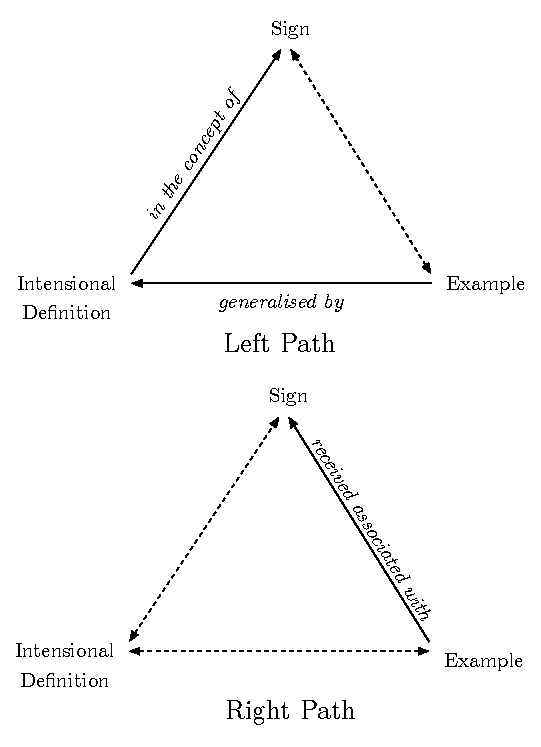
\includegraphics[width = 200pt]{figs/paths.pdf}
    \caption{Paths of example-sign associations offered to the agents. The right path is considered as the "objective truth" as it has been received by the oracle, while the left path is an inference made through learning that can be used in a more diverse set of scenarios to make new associations.}
    \label{fig:path}
\end{figure}

% Oracle distribution
In the case of a two-agents alignment scenario, the oracle can give different set of example signs associations for the agents to learn over. From now, I will consider that the general case is indeed $U_{k} \prescript{}{o}{\mapsto} S_{k} \neq U_{-k} \prescript{}{o}{\mapsto} S_{-k}$. The differences between $U_{k} \prescript{}{o}{\mapsto} S_{k}$ and $U_{-k} \prescript{}{o}{\mapsto} S_{-k}$ are responsible for most of the issues that are present in classifier alignment. Note that we keep using the notation  $U_{k} \prescript{}{o}{\mapsto} S_{k}$ for the set of associations received from the oracle, since the oracle does not use paths to make these associations. On the contrary, the generic set of received associations of $A_{k}$ is noted $U_{k} \prescript{r}{k}{\mapsto} S_{k}$ since all these associations are indeed right-path associations when they are made by $A_{k}$.

% Definition of homogeneity
The notions of left-path associations and right-path associations gives a better presentation of the role of learning and allows us to define the homogeneity of a set properly. As mentioned before, this definition is presented below:

\begin{restatable}[Homogeneity]{df}{Homogeneity}
\label{def:Homogeneity}
Let $A_{1}$ and $A_{2}$ be two agents. A set of example-sign associations $U \mapsto S$ is considered as homogeneous if, for any pair of its subsets $U_{1} \mapsto S$ and $U_{2}\mapsto S$ such that $(U_{1} \mapsto S) \cup (U_{2} \mapsto S)$, we have $U_{k} \prescript{l}{A1}{\mapsto} S = U_{k} \prescript{l}{A2}{\mapsto} S$.
\end{restatable}

Of course, a learning can be non-deterministic and often admits a degree of error, this is why we prefer to speak about a degree of homogeneity instead of a strict homogeneity. The degree of homogeneity is defined below:

\begin{restatable}[Degree of homogeneity]{df}{DoHomogeneity}
Let $A_{1}$ and $A_{2}$ be two agents. The degree of homogeneity $d_{h}$ of two sets of example-sign associations $U_{1} \mapsto S$ and $U_{2} \mapsto S$ is given by the formula:

\[
d_{h} = \frac{1}{2} \sum_{k = 1}^{2} \frac{|U_{k} \prescript{l}{A1}{\mapsto} S \cap U_{k} \prescript{l}{A2}{\mapsto} S|}{|U_{k} \mapsto S|}
\]

\end{restatable}

\section{Issues in Classifier alignment}

\subsection{Predictable issues in classifier alignment}
% Predictable issues linked to classifier alignment
The initial situation in which two classifier agents receive different sets of associations and learned over them. The possible differences between the result of this learning on the knowledge of these agents and the final state expected from these agents in order to have a classifier alignment allows us to make predictions on the issues that are linked to classifier alignment. While we have already mentioned that the general case is $U_{k} \prescript{}{o}{\mapsto} S_{k} \neq U_{-k} \prescript{}{o}{\mapsto} S_{-k}$, the types of differences between these two sets of associations allow us to classify the issues in alignment into main families, that we call situations of alignment.

% Agents might not share their examples
\paragraph{Different examples distributed:} The two sets of associations distributed by the oracle can be different simply because the examples that the agents receive are different. In this case, $U_{k} \neq U_{-k}$. The main issue associated with this case, is that the agents cannot use the right-path to associate a sign to the examples of the other agent since the examples from $U_{-k} - U_{k}$ are not found in $U_{k} \prescript{}{o}{\mapsto} S_{k}$. A more problematic issue is that it becomes hard to compare the classifications of the two agents, since their partitions are not the same: the class $U(\prescript{l}{k}{\mapsto} s)$ is likely to have different examples from the class $U(\prescript{l}{-k}{\mapsto} s')$ with both classes having their own particular examples. While this issue does not affect a naming game that uses the left-path to associate signs with presented examples, we will see later that this issue has a real impact when we will have to define a notion of equivalences between the concepts of different agents. Unfortunately, this case is the general case in machine learning and multi-agent systems, and is the only case considered in thesis. In the rest of the thesis, the sets of examples $U_{-k} - U_{k}$ and $U_{k} - U_{-k}$ are always non-empty, granting each agents with their own separate knowledge.

% Agents might not share their signs
\paragraph{Different signs distributed:} The two sets of associations distributed by the oracle can also be different because the signs that the agents received are different. In this case, $S_{k} \neq S_{-k}$. The main issue associated with this case is that even if two classes $U(\prescript{l}{k}{\mapsto} s)$ and $U(\prescript{l}{-k}{\mapsto} s')$ are equal, the agents will associate a different signs to their example and while the agents are sharing the partition of their examples, they are unable to pass the naming game.

% Agents might not share their example signs associations
\paragraph{Distinct example-signs associations} The two sets of associations are distributed by the oracle can share the same examples and the same signs, but still have different example-sign associations. In this case,  $U_{k} = U_{-k}$ and $S_{k} = S_{-k}$, but $U_{k} \prescript{}{o}{\mapsto} S_{k} \neq U_{-k} \prescript{}{o}{\mapsto} S_{-k}$. In the previously discussed cases, we could always imagine that there were one set of associations $U \prescript{}{o}{\mapsto} S$ that was distributed among the agents -- not the same associations in the case of the different examples distributed, and by substituting the signs of some classes in the case of different signs distributed, but we could always track the two sets distributed back to one set of associations that had classes. In the present case, it would be impossible without associating more than one sign associated to some examples. This case is better understood as if the oracle was distributing two distinct sets of associations instead of one to the classifier agents.

% Agents might not have their two paths making the same associations locally
\paragraph{Distinct local-path associations} The two agents have received the same set of associations and $U_{1} \prescript{}{o}{\mapsto} S_{1} = U_{2} \prescript{}{o}{\mapsto} S_{2}$. However, at least one of the agent $A_{k}$ did not succeed to make an accurate learning over the set $U_{k} \prescript{}{o}{\mapsto} S_{k}$. The consequence is that $U_{k} \prescript{l}{k}{\mapsto} S_{k} \neq U_{k} \prescript{r}{k}{\mapsto} S_{k}$. If the agents use the right path to name the examples that are presented to them during the naming game, this case is without incidence. However, if the agents use the left path to name the examples -- and we have already shown that the left-path should be the preferred path to make associations -- the agents will probably produce some errors. Indeed, a situation where the learning errors of $A_{k}$ and $A_{-k}$ are nullifying each others such that $U_{1} \prescript{l}{k}{\mapsto} S_{1} = U_{2} \prescript{l}{-k}{\mapsto} S_{2}$ is highly unlikely to happen.

% Agents might not associate one sign to one example
\paragraph{Unknown association and Multiple associations} Depending on the algorithm used for the supervised learning, an agent $A_{k}$ can end up with either none or more than one sign associated to one example - either an example from its local context $U_{k}$ in the case of an inaccurate learning, or an example presented later during the naming game, or an example exchanged with the agent $A_{-k}$. This can be the case in my thesis, since I use inductive learning and cannot guarantee that only one of the generalizations that come as the output of my learning are subsuming disjoint sets of examples in any context -- or that for any possible example, one of the learned generalization will subsume it.


\subsection{Classes of alignment situations}

% Presenting the issue with the combination of different cases
The issues that are listed in the previous section are not all mutually exclusive, and often a situation combines two or more of them. Even for mutually exclusive cases, some aspects of a case can be combined with some aspects of another in order to create a hybrid case. In my scenarios for instance, the examples that are received by the agents as learning sets are always at least partially different. What differentiates my scenarios are the other cases that are combined with the \emph{different examples distributed} case. As a direct consequence of this, the fact that the agents are not receiving the same examples at the beginning often masks issues that would have been better understood if they had received the same examples. For this reason, we need to look at these issues from the point of view of the oracle, and see how these issues are perceived by the agents after the distribution.

% Distinguish cases due to the learning and cases independent from the learning
Looking at the five cases of predictable issues listed in the section above, we can see that the three first cases of issues are independent of the agent's learning while the two lasts are caused by the learning inaccuracies or intrinsic limitations. In this section, we will see that it is sometime complicated to identify if a situation that causes issues in the classifiers alignment is due to the agents' learning or if the problem is totally independent. This information is however essential for the agents: an issue caused by an error in the learning can be corrected with the agents sharing their knowledge and learning again a more accurate set of generalizations. However, if the issue is not caused by the learning, the agents will need to question the nature of the information they have in order to overcome their disagreements.

\begin{figure}[t]
    \centering
    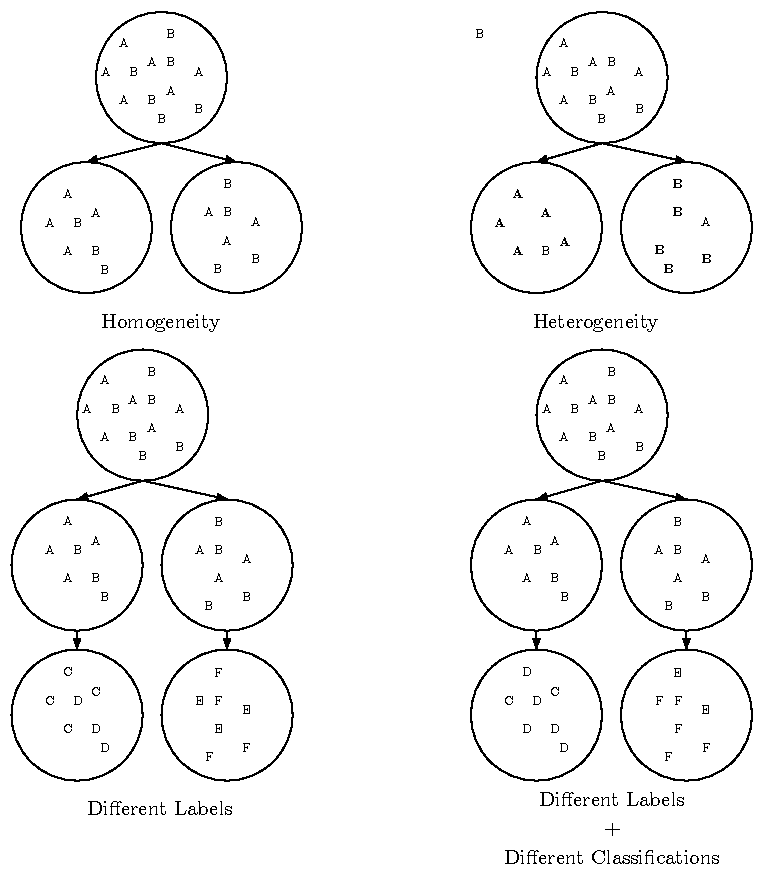
\includegraphics[width = 250pt]{figs/different_situations.pdf}
    \caption{The different situations of classifier alignments. The top circle always represent the hypothetical set of associations that the oracle is supposed to have access to. The letters represent the examples and their associated signs. The oracle's set of associations is either directly distributed among the agents (top line), or they go through a step of distribution and a state of alteration of the classes (bottom line).}
    \label{fig:classProblem}
\end{figure}

% Introduction to situations
The different combinations of cases, called situations, are presented below. In each situation, the local contexts $U_{1}$ and $U_{2}$ are different. Of course, situations can be combined as well in order to make hybrid situations. The situations are illustrated in Figure \ref{fig:classProblem}, and will be presented below as they appear on this figure from left to right.

% Homogeneity situation
\subsubsection{Homogeneity situation} The situation is homogeneous when the oracle has a unique and consistent set of associations $U \prescript{}{o}{\mapsto} S$ and gives to $A_{1}$ and $A_{2}$ different subsets of $U \prescript{}{o}{\mapsto} S$. In this scenario, the subsets receive associations from each class of $U \prescript{}{o}{\mapsto} S$ in similar proportion, which facilitates the classifier alignment. Indeed, the generalizations that will be learned over sets of examples of similar sizes are likely to be similar themselves, and we can expect to have $U \prescript{l}{A1}{\mapsto} S \approx U \prescript{l}{A2}{\mapsto} S$. Therefore, we can expect to observe a high score from $A_{1}$ and $A_{2}$ on a naming game that takes place over the context $U$, or even different contexts. The homogeneity is the most ideal distribution of examples that can take place in a situation where $U_{1} \prescript{}{o}{\mapsto} S \neq U_{2} \prescript{}{o}{\mapsto} S$.

% Heterogeneity situation
\subsubsection{Heterogeneity situation} The situation is heterogeneous when the oracle still has a unique and consistent set of associations $U \prescript{}{o}{\mapsto} S$ and gives to $A_{1}$ and $A_{2}$ different subsets of $U \prescript{}{o}{\mapsto} S$, but this time the agents receive associations from the classes of $U \prescript{}{o}{\mapsto} S$ in different proportions. The issue here is that the generalizations are likely to be different from one agent to another, even for a same classes, due to a lack of precision for the agent that has received the least examples of that class. Even if $U_{1} \prescript{l}{A1}{\mapsto} S \approx U_{1} \prescript{r}{A1}{\mapsto} S$ and $U_{2} \prescript{l}{A2}{\mapsto} S \approx U_{2} \prescript{r}{A2}{\mapsto} S$, the difference in composition between $U_{1}$ and $U_{2}$ are likely to cause $U \prescript{l}{A1}{\mapsto} S \neq U \prescript{l}{A2}{\mapsto} S$.

% Different signs situation
\subsubsection{Different signs situation} The situation of different signs is also based on the case of different examples distributed, but this time mixed with the case of different signs distributed. As for the situations of homogeneity and heterogeneity, we can imagine the oracle distributing the associations of a consistent set of associations $U \prescript{}{o}{\mapsto} S$ between two sets of associations, $U_{1} \prescript{}{o}{\mapsto} S$ and $U_{2} \prescript{}{o}{\mapsto} S$. However this time, before giving these sets of associations to the two agents, the oracle is replacing the lexicon $S$ of these sets by two new separate lexicons $S_{1}$ and $S_{2}$. In this situation, the classes are not modified: if the sign $s \in S$ has been replaced by the sign $s_{k} \in S_{k}$, we observe the equality $U(\prescript{}{o}{\mapsto} s) = U(\prescript{}{o}{\mapsto} s_{k})$. The fact that $U_{1}(\prescript{}{o}{\mapsto} s_{1}) \neq U_{2}(\prescript{}{o}{\mapsto} s_{2})$ is imputable to $U_{1} \neq U_{2}$, not to $S_{1} \neq S_{2}$. In this situation, the set of associations $(U_{1} \prescript{}{o}{\mapsto} S_{1}) \cup (U_{2} \prescript{}{o}{\mapsto} S_{2})$ is not consistent, but each of its example is associated with exactly one pair of signs: one sign from $S_{1}$ and one sign for $S_{2}$. Additionally , if an example from the set $(U_{1} \prescript{}{o}{\mapsto} S_{1}) \cup (U_{2} \prescript{}{o}{\mapsto} S_{2})$ is associated with two signs $s_{i} \in S_{k}$ and $s_{j} \in S_{-k}$, then there cannot be another example $e'$ from the same set associated to a pair of signs $s_{i} \in S_{k}$ and $s_{l}' \in S_{-k}$ such that $s_{j} \neq s_{l}$.

% Different classifications situation
\subsubsection{Different classifications situation} The situation of different classifications is base on the case of different examples distributed. In this situation, the union $U_{1} \prescript{}{o}{\mapsto} S_{1} \cup U_{2} \prescript{}{o}{\mapsto} S_{2}$ does not form a consistent set of consistent example-sign associations. While this was also the case in the situation of different signs, this time there is no relation of equivalence between the classes of $U_{1} \prescript{}{o}{\mapsto} S_{1}$ and $U_{2} \prescript{}{o}{\mapsto} S_{2}$. In this situation there can be an example from the set $(U_{1} \prescript{}{o}{\mapsto} S_{1}) \cup (U_{2} \prescript{}{o}{\mapsto} S_{2})$ that is associated with two signs $s_{i} \in S_{k}$ and $s_{j} \in S_{-k}$, and a second example $e'$ that is associated with another pair of signs $s_{i} \in S_{k}, s_{l} \in S_{-k}$ such that $s_{j} \neq s_{k}$. Intuitively, it does not seem that this situation can be explained as the distribution of a consistent set of associations, but rather as the oracle presenting two unrelated sets of associations to the agents. However, we can imagine that there exists a consistent set of associations $U \prescript{}{o}{\mapsto} S$ that has been distributed in two subsets $U_{1} \prescript{}{o}{\mapsto} S$ and $U_{2} \prescript{}{o}{\mapsto} S$ such that $U_{1} \neq U_{2}$, that are therefore consistent as well -- so far, this in an homogeneous situation. In order to explain how two examples that belong to a same class in $U_{k} \prescript{}{o}{\mapsto} S_{k}$ can belong to two different classes in  $U_{-k} \prescript{}{o}{\mapsto} S_{-k}$, we can imagine that some of the classes from one set $U_{k} \prescript{}{o}{\mapsto} S_{k}$ has been merged together. A merge between two classes $U(\prescript{}{o}{\mapsto} s_{i})$ and $U(\prescript{}{o}{\mapsto} s_{j})$ of the set of associations $U_{k} \prescript{}{o}{\mapsto} S_{k}$ is done by removing the set of associations of the two classes, $U(\prescript{}{o}{\mapsto} s_{i}) \prescript{}{o}{\mapsto} s_{i}$ and $U(\prescript{}{o}{\mapsto} s_{j}) \prescript{}{o}{\mapsto} s_{j}$, and replacing them by a new set of associations $(U(\prescript{}{o}{\mapsto} s_{i}) \cup U(\prescript{}{o}{\mapsto} s_{j})) \prescript{}{o}{\mapsto} s_{l}$ that associates the union of the two classes merged to a same sign $s_{l}$. Since the number of classes changes each time that a merge occurs, the sizes of the lexicons change as well as they become different. Then, the resulting sets of associations are given to the agents as $U_{1} \prescript{}{o}{\mapsto} S_{1}$ and $U_{2} \prescript{}{o}{\mapsto} S_{2}$.

\section{Reaching Mutual Intelligibility}

% Introduction
The details of our approach to reach mutual intelligibility will be addressed later in the thesis, with the proper notation. However, we can already discuss generalities on how multi-agent systems can align themselves.
% Alignment is in fact left path alignment
The first thing that should be decided over the alignment, is if we want a left-path or a right-path alignment, or a mix of the two. Indeed, the agents have two different paths to associate a sign with an example and therefore can name a presented example with more than one path on certain conditions. The problem is that these paths, as we mentioned before, might not make the same associations. Therefore, the first thing that an agent should know in order to play the naming game is which path should be used when. While the right-path represent a knowledge obtained from the oracle and therefore deemed as more accurate, the right-path can only help to name examples that are part of the examples received from the oracle. This limitation forces the agent to prefer the left-path for most of the examples involved in the naming game. Of course, an agent could use the right-path by default and resort to the left-path only for examples that it has not receive from the oracle, but mixing paths in the naming game can be problematic: for instance, in the case of agents arguing, there is a risk that an agent names an example with a sign that seems inconsistent with the generalizations and arguments that this agent has shared with the other agent. We call this left-path alignment \emph{mutual intelligibility}.

\subsection{Reaching mutual intelligibility according to the situation}

\subsubsection{Homogeneity and heterogeneity} The situation of homogeneity should not cause any problem and the classifiers should already be quasi-aligned after the supervised learning. The situation of heterogeneity is close to the one of homogeneity, but induces more overlaps between the left-path associations of the two agents. We can in fact consider that a situation of homogeneity becomes a situation of heterogeneity not when a threshold is reached in the imbalance of examples between classes of the two agents, but when the left-path associations of the two agents are resulting in too many errors during the naming game for the agents to consider that their learning data-sets where homogeneous. In these two situations, the agents could just exchange all of their example-sign associations to find the original set of associations $U \prescript{}{o}{\mapsto} S$ that is the union of their two local sets. With this overall set of associations, the agent could learn new generalizations for their left-path associations without difficulty, since as we mentioned the overall set of associations is consistent. Of course, transferring all the examples from one agent to another is costly in term of information exchanged examples. This is were algorithms such as Amail intervene: they use arguments that summarize the information of chosen subsets of the local sets of associations, and allow the agents to reduce the volume of information that they need to exchange in order to align their left-path associations.

\subsubsection{Different signs} The situation of different signs is radically different the the homogeneity and heterogeneity situation. An algorithm like Amail could not directly be used in this situations, since the union of the two local sets of example-sign associations of the agents is not a consistent set of associations. Therefore, it cannot be used as a learning set for supervised learning by the agents. This means that even if the agents were to exchange all of their example-sign associations, they could not anything that would help them to pass the naming game. However, since the classes of the agents are mapped one to one, the agents can make a pre-processing \emph{before} using Amail.
% The mapping
In this pre-processing, the agents will find correspondences between their classes by examining which of them are equivalent. Of course, since the agents have different examples, the classes from different agents are almost always expected to be different -- it is the case in any scenario. However, the agents can look at the equivalence in the overall context $U_{1} \cup U_{2}$, by finding the pairs of classes $(U_{1} \cup U_{2}) \prescript{l}{A1}{s_{i}}$, $(U_{1} \cup U_{2}) \prescript{l}{A2}{s_{j}}$ are having the same examples. We call this process a \emph{mapping} of the classes of the two agent. The agents can do this mapping by exchanging all of their examples to have both access to the overall context, but if they want to limit the amount of information exchanged they can use ontology matching algorithms in order to make a one-to-one mapping of their classes.
% From mapping to a situation of homogeneity or heterogeneity
Once the classes are mapped, the agents can change the signs associated to the examples of these classes -- that should be two different signs per matching classes, one from each agent's lexicon -- to a common sign per matching classes. Once this is done, the agents are finally using the same lexicon. The union of the two agents' sets of associations is now a consistent set, and the agents are in a situation of homogeneity or heterogeneity on which algorithms like Amail can make the agents reach mutual intelligibility.

\begin{figure}
    \centering
    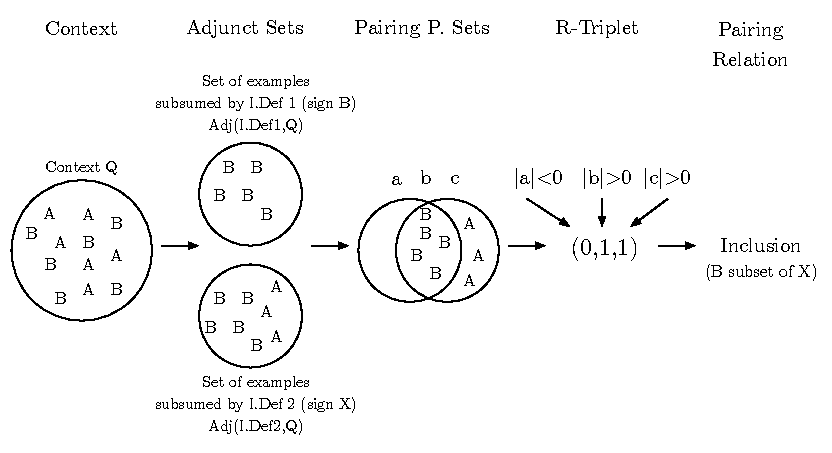
\includegraphics[width = 250pt]{figs/5.pdf}
    \caption{Relation between the context, concepts' adjunct sets, pairing partial sets, r-triplets and pairing relations. The left-path (intensional definitions) partitions a context into adjunct sets. Two adjunct sets create three theoretical pairing partial sets. The count of examples in each pairing partial sets gives the r-triplet of the relation between the two adjunct sets. The r-triplet gives the quality of the pairing relation of the concepts from with the left-paths have been borrowed to make adjunct sets.}
    \label{fig:pRelations}
\end{figure}

\subsubsection{Different classifications} The situation of different classifications is comparable to the situation of different signs in the sense that the union of the two local set of associations of the agents cannot make a consistent contrast-set. However, unlike the situation of different signs, there is no possible one-to-one mapping between the classes of the agents and this is why there is no pre-processing that can turn this situation into something compatible with Amail without seriously altering the classes of both agents, as learning and argumentation is only useful if the agents are learning and arguing within an overall set of relations that is consistent. There can be two approaches to overcome this problem.
% How did we get there
We mentioned that this situation is analog to an oracle distributing the associations of a consistent set of associations $U \prescript{}{o}{\mapsto} S$ among two subsets $U_{1} \prescript{}{o}{\mapsto} S$ and $U_{2} \prescript{}{o}{\mapsto} S$, and then merge differently the classes of each of these two sets in order to obtain two new sets $U_{1} \prescript{}{o}{\mapsto} S_{1}$ and $U_{2} \prescript{}{o}{\mapsto} S_{2}$.
% Create a mapping
After the merge, it is impossible for the agents to make a one to one mapping of their class since they might even differ in number from one agent to another. Instead of doing a one-to-one mapping based on a relation of equivalence between the classes, the agents can do a all-to-all mapping using \emph{pairing relations}. Unlike the relation of equivalence that can only map two classes $(U_{1} \cup U_{2}) \prescript{l}{A1}{s_{i}}$ and $(U_{1} \cup U_{2}) \prescript{l}{A2}{s_{j}}$ if they have the same examples, the pairing relations can map these two classes no matter how many examples they have in common. The information about these classes having examples in common is stocked as r-triplets. The relation between pairing relations, r-triplet and the sets of examples shared by the two classes (called pairing partial sets) is presented in Figure \ref{fig:pRelations}. As Amail was useful to spare information transfer in situations of heterogeneity, and ontology-matching algorithms were useful to spare information transfer in situations of different signs, the argumentation model that I propose comes with a process that spares information in the different classifications situations when it comes to identify the pairing partial sets, r-triplets and pairing relations of the agents.
% Reverse the merge
Once the mapping is done, the agents have all the information they need to identify the classes that have been merged in $U_{1} \prescript{}{o}{\mapsto} S$ and $U_{2} \prescript{}{o}{\mapsto} S$. By splitting their classes, the agents can reverse the process of merging that theoretically occurred in the two sets $U_{1} \prescript{}{o}{\mapsto} S$ and $U_{2} \prescript{}{o}{\mapsto} S$. The splits result in a class for each pairing partial set that were present in the mapping; a pairing partial set can also be seen as a class $(U_{1} \cup U_{2})(\prescript{l}{k}{\mapsto} s_{i},s_{j})$ of the union of the two local sets of associations. Therefore, there will be a new class for each different pair of signs that can be find in the union of the two local sets of associations.
% Make a one to one mapping
Once the split has been done, the agents have a new set of classes. Since there is a new class for each pair of signs that are associated to examples in the union of the two sets of associations, the agents can now make a one to one mapping of their classes. The agents have reached a situation of different signs. The agents can, by using an ontology alignment algorithm, reach a situation of heterogeneity or homogeneity.
% Again, we are in a situation where we can use Amail
Once in a situation of heterogeneity or homogeneity, the Amail algorithm can be use to reach mutual intelligibility over the overall context of the agents.

\subsection{Identifying the Situation}

In the previous section, we have detailed how to move from each situation to a situation of homogeneity where the agents share enough information to learn intensional definitions that are allowing mutual intelligibility. The path followed through the simplification of these situations is illustrated in Figure \ref{fig:simplification}.

\begin{figure}
    \centering
    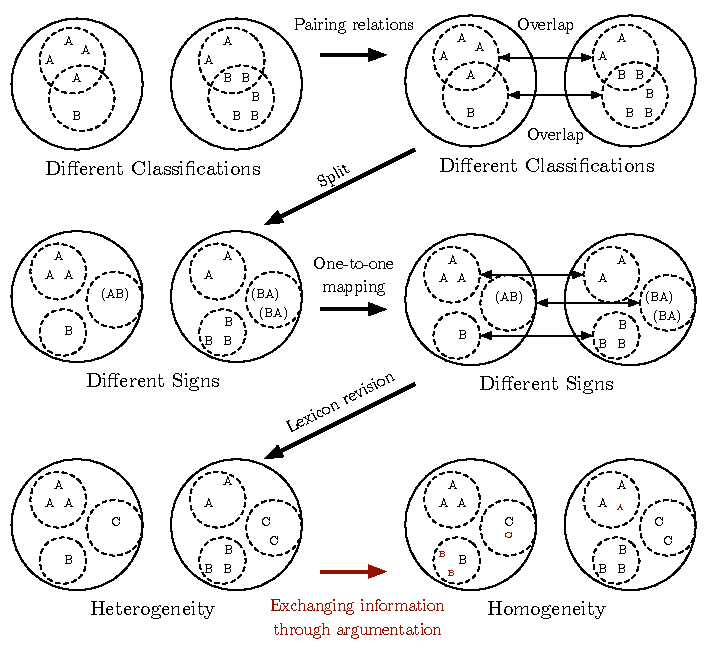
\includegraphics[width = 250pt]{figs/situations_simplification.pdf}
    \caption{The simplification of each situation into a simpler one, each time presented with the method used.}
    \label{fig:simplification}
\end{figure}

However, the agents have no \emph{a priori} knowledge on which scenario they are when they meet each other and try to reach mutual intelligibility. Therefore, before using any method to simplify their current situation they need to figure out which is their actual current situation.

% Why we are in a different paradigm when we try to solve and when we try to identify a situation
The problem with the identification of the situations, is that we are classifying them according to a narrative that is just an abstract justification for the differences between the agents' classifications. This narrative of an oracle that distributes the examples of a consistent set of associations among two subsets might or might not have a reality in our scenarios, as the experimenter might follow these steps to create the training set of the examples or use two already-different training sets. In the latter scenario, we can always imagine that the two already-different training sets are parts of a reality that can be seen as a consistent set of associations, if we chose to put ourselves in a constructivist paradigm. However, all these steps are hypothetical and we only presented them to produce a reverse model of this narrative that leads to a consistent set of associations where there are actually two sets that seems to contain at least some inconsistent information. While understanding this idea is important to present how to reach mutual intelligibility in each different situation, it has no use to try to guess in which situation are the agents.

% Since we cannot access the narration that led to the creation of these two sets, we should look at the effect that this narration has
The narration of the situation's creation is hypothetical, and even in cases where it is not, the agents cannot directly access it. Therefore, the identification of the different solutions requires to look for the effects of this narration over the sets of associations of the agents.

%% Effect on the right path associations
\subsubsection{Effect on the right-path associations}

\begin{figure}
    \centering
    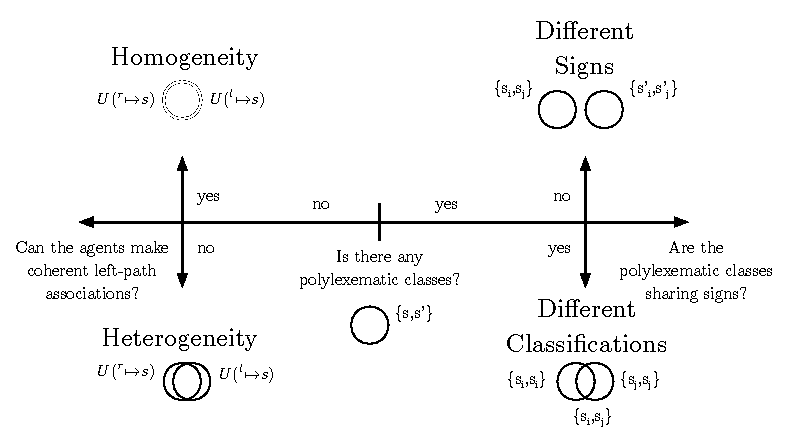
\includegraphics[width = \textwidth]{figs/situations_id_r.pdf}
    \caption{Identification of the agents' situation based on right-path associations comparison.}
    \label{fig:r_situation_id}
\end{figure}

% The creation of situations affects primarily the right path associations
The creation of the local training sets of associations is only involving the right-path associations, since the associations given by the oracle to the agents at the start of any scenario are treated as right-path associations.
% Can check the presence of polylexematic classes
Identifying the situation is trivial if the agents have access to both $(U_{1} \cup U_{2}) \prescript{r}{A1}{\mapsto} S_{1}$ and $(U_{1} \cup U_{2}) \prescript{r}{A2}{\mapsto} S_{2}$. The agents are by definition in a situation of homogeneity or heterogeneity if and only if the union of these two local sets of associations are consistent. This verification splits the situations in two classes, that we will call consistent and inconsistent situations. The consistent situations are the homogeneity and heterogeneity situations, while the inconsistent situations are the different signs and different associations situations. Once the agents have determined if the situation is consistent or inconsistent by checking the union of their local sets of associations, they can determine for each class which of the two situations inside is their current situation.

% homogeneity vs heterogeneity
If the agents determined that their situation is a consistent relation, they can use their supervised learning over their respective local sets of associations to see if they obtain the same generalizations. If this is the case, then the information has been homogeneously distributed between their training sets and they are in a homogeneous situation. On the contrary, if the generalizations over the two local training sets classify the other agent's training set with differences compared to the right-path associations, the agents know that they are in a situation of heterogeneity.

% different signs vs classifications
If the agents have found polylexematic classes in the union of their local training sets, they know that they are either in a situation of different signs or different classifications. By looking at the different set of signs associated to each of the classes, the agents can determine in which situation they are. There can exist two classes $(U_{1} \cup U_{2})(\prescript{r}{}{\mapsto} \{s_{i},s_{j}\})$ and  $(U_{1} \cup U_{2})(\prescript{r}{}{\mapsto} \{s_{i}',s_{j}'\})$ such that $s_{i} = s_{i}'$ but $s_{j} \neq s_{j}'$, if and only if the agents are in a situation of different classifications. Therefore, there are no such pair of classes in the union of the two training sets, the agents know that they are in a situation of different signs.

% Problem with creating a set of right-path associations that can allow this identification
The problem with this identification method is that it requires the agents to create the set of associations $((U_{1} \cup U_{2}) \prescript{r}{A1}{\mapsto} S_{1})$ $\cup$ $((U_{1} \cup U_{2}) \prescript{r}{A2}{\mapsto} S_{2})$. A set of association $(U_{1} \cup U_{2}) \prescript{r}{k}{\mapsto} S_{k}$ can exist only if the agent $A_{k}$ has received it as its initial training set, or in other words if its initial training set contained all the examples from $U_{1}$ and $U_{2}$ -- which is the same as saying that $U_{1} = U_{2}$. Since this is a particular case, the agents are not able to use their right path associations to identify their situation in the general case.

%% Effect of the left path associations
\subsubsection{Effect on the left-path associations}

% Then the only option left is the left path associations
Since comparing the right-path associations of the agents has been ruled out, the agents can only compare their left-path associations if they want to determine their situation. In order to determine which are the effects of the distribution process over the different situations, we will take as a reference the homogeneous situation and consider the three other situations as variations. Then we can observe the effect of each variation on the differences between the left-path associations of the two agents.

% Ideal sets are homogeneous sets
The ideal sets are homogeneous. If the sets are homogeneous, the agents can substitute the 

% Each other situation is a deviation from the homogeneous situation

% The heterogeneous is (-) information shared

% The different signs is (-) lexicon shared

% The different classifications is (-) classes shared

% Each of the three deviations have the same impact: union of the two sets with polylexematic classes

\section{Argumentation and example exchanges}